\documentclass[12pt]{article}
\usepackage[T1]{fontenc}
\usepackage{calc}
\usepackage{setspace}
\usepackage{multicol}
\usepackage{fancyheadings}
 
\usepackage{graphicx}
\usepackage{color}
\usepackage{rotating}
\usepackage{harvard}
\usepackage{aer}
\usepackage{aertt}
\usepackage{verbatim}
\usepackage{array}
\usepackage{multirow}

\setlength{\voffset}{-0.25in}
\setlength{\topmargin}{0pt}
\setlength{\hoffset}{0pt}
\setlength{\oddsidemargin}{0pt}
\setlength{\headheight}{0pt}
\setlength{\headsep}{.4in}
\setlength{\marginparsep}{0pt}
\setlength{\marginparwidth}{0pt}
\setlength{\marginparpush}{0pt}
\setlength{\footskip}{.1in}
\setlength{\textwidth}{6.5in}
\setlength{\textheight}{9.25in}
\setlength{\parskip}{0pc}

\renewcommand{\baselinestretch}{1.5}

\newcommand{\bi}{\begin{itemize}}
\newcommand{\ei}{\end{itemize}}
\newcommand{\be}{\begin{enumerate}}
\newcommand{\ee}{\end{enumerate}}
\newcommand{\bd}{\begin{description}}
\newcommand{\ed}{\end{description}}
\newcommand{\prbf}[1]{\textbf{#1}}
\newcommand{\prit}[1]{\textit{#1}}
\newcommand{\beq}{\begin{equation}}
\newcommand{\eeq}{\end{equation}}
\newcommand{\bdm}{\begin{displaymath}}
\newcommand{\edm}{\end{displaymath}}
\newcommand{\script}[1]{\begin{cal}#1\end{cal}}
\newcommand{\citee}[1]{\citename{#1} (\citeyear{#1})}
\newcommand{\h}[1]{\hat{#1}}
\newcommand{\ds}{\displaystyle}
\newcommand{\normal}{\mathcal{N}}
\newcommand{\centerpic}[2]{\begin{center}\includegraphics[#1]{#2}\end{center}}

\pagestyle{empty}



\begin{document}

\section{Summary}
\bi
\item While analyzed separately, a casual look at both pitcher and hitter salary data shows they exhibit similar behavior, climbing above and falling below the long-run growth trend at similar times.
\item The model very strongly predicts regime switching behavior for both hitters and pitchers.  Estimated probabilities for being in one regime or the other are very close to 1.0 for every time period.
\item While analyzed separately, both pitchers and hitters regime changing behavior is very similar.
\item In the OLS regressions, all variables have statistically significant coefficients.  In both regressions and in all regimes, all coefficients have the expected sign.
\item Regimes are very persistent.  The league begins in regime 2 at the onset of free-agency until the early to middle 1980s.  The league remains in regime 1 from the early 1980s through the early 2000s.
\item The time period from the early 1980s through early 2000s (regime 1) largely coincides with the average salary above its long-run steady state growth path.  
\item In the regime switching regression results for both pitchers and hitters, regime 1 is characterized by a statistically significant lower exogenous average trend growth rate (negative difference on time).
\item In the regime switching regression results for pitchers, regime 1 is characterized by less reward for performance variables including wins, saves (statistically significant), and SO/BB (not statistically significant).
\item In the regime switching regression results for hitters, including only OPS x AB (On-base percentage + Slugging Average) x (At Bats) leads to no statistically or economically significant difference in this coefficient between regimes (results not shown).  Adding the home run variable leads to an interesting conclusion (results shown in Table 2).  Regime 1 is characterized by higher reward for performance as measured by OPSxAB (statistically significant), but less reward for home runs (though this is not statistically significant).  Therefore, in Regime 2 (before early 1980s and after early 2000s), salary becomes more dependent on home run output and less so on the broader measure of player performance (OPS x AB).
\item For both hitters and pitchers, there appears to be little difference between regimes in the evolution of salary based on age or experience.  This is true even though the experience term is statistically significant in the pitchers regression.  Upon computing the years of experience in which pitchers reach their peak salary, the differences are not economically meaningful (16.9 years versus 17.0 years).
\item Pseudo R-squared values.  In each set of regressions, this is the percentage of salary data that remains unexplained in the ordinary least-squares procedure (after taking into account all of the explanatory variables in a traditional fashion) that we are able to explain by allowing for regime switching.  That is, this is a measure of the improvement in explanatory power deriving from simply allowing switching in the regression coefficients, but not actually bringing in any more information or variables into the model.  For pitchers this is about 9\% and for hitters this is about 5\%. 
\ei
\newpage

\begin{figure}\caption{Average Salary 1976 - 2007}
\begin{center}
\begin{tabular}{cc}
\textbf{Pitchers} & \textbf{Hitters} \\\\
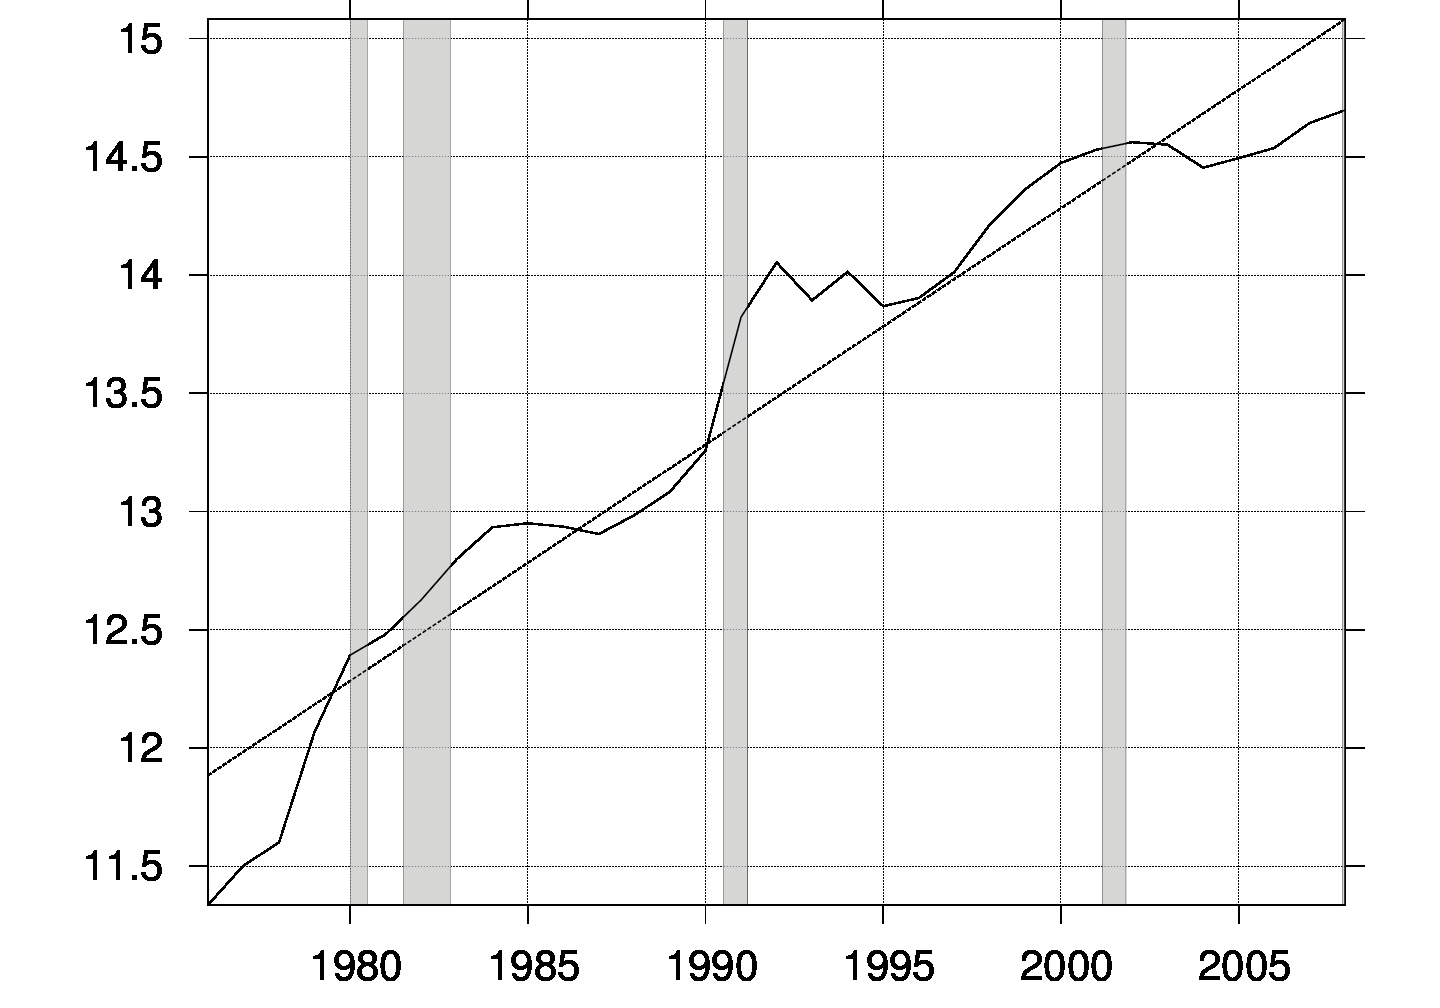
\includegraphics[scale=0.16]{pitchers/logfitsals.png} & 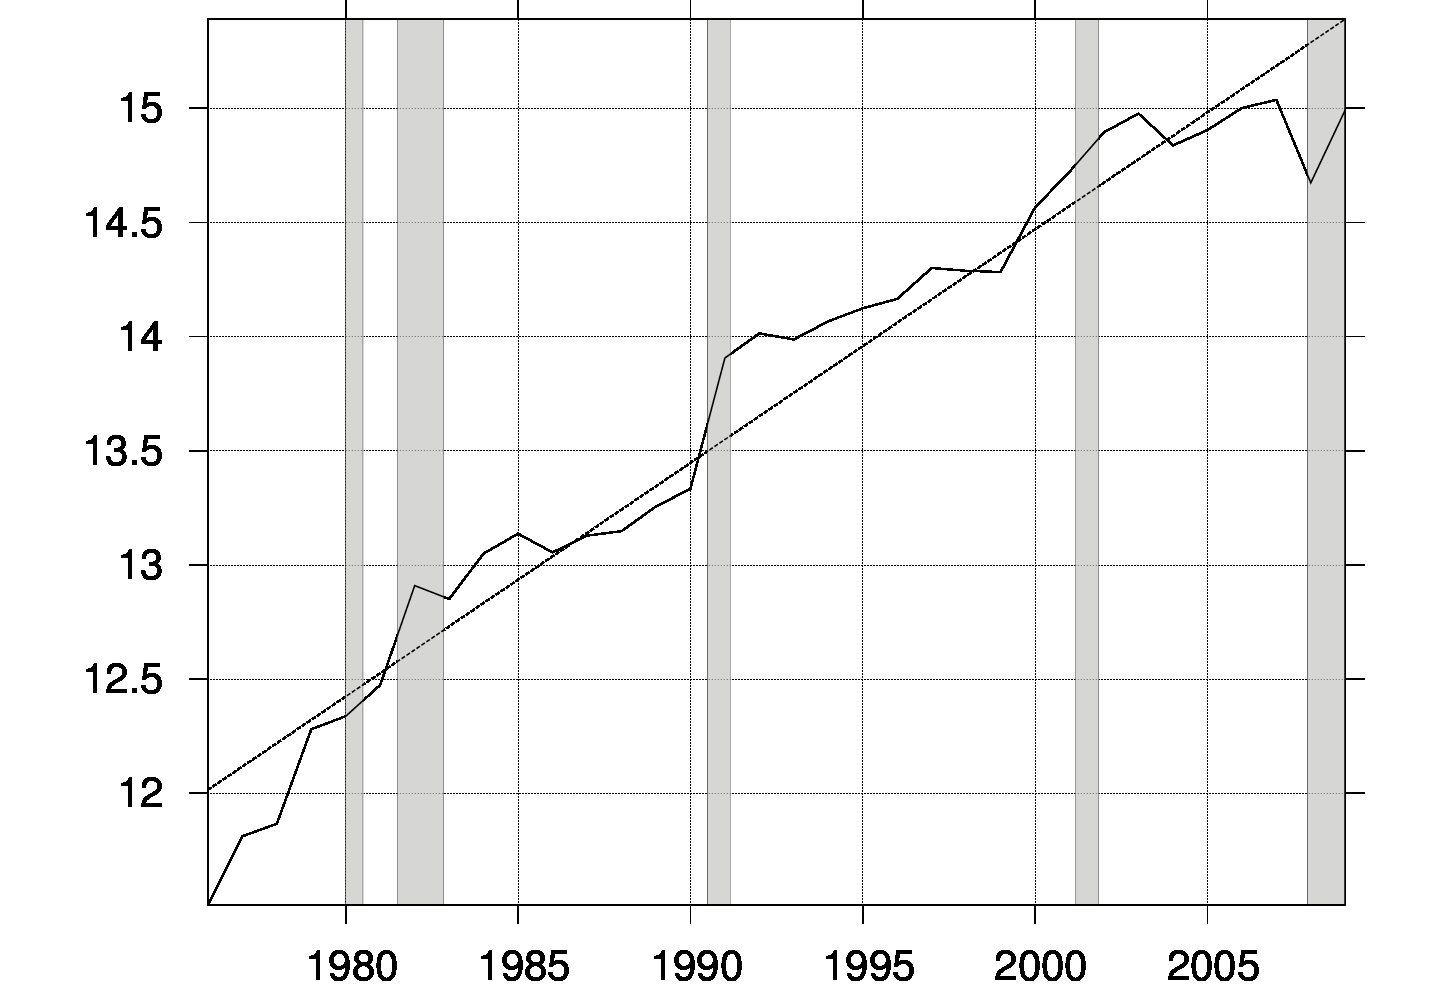
\includegraphics[scale=0.16]{hitters/logfitsals.png} \\
\multicolumn{2}{c}{Log-Salaries with Linear Trend Line} \\\\
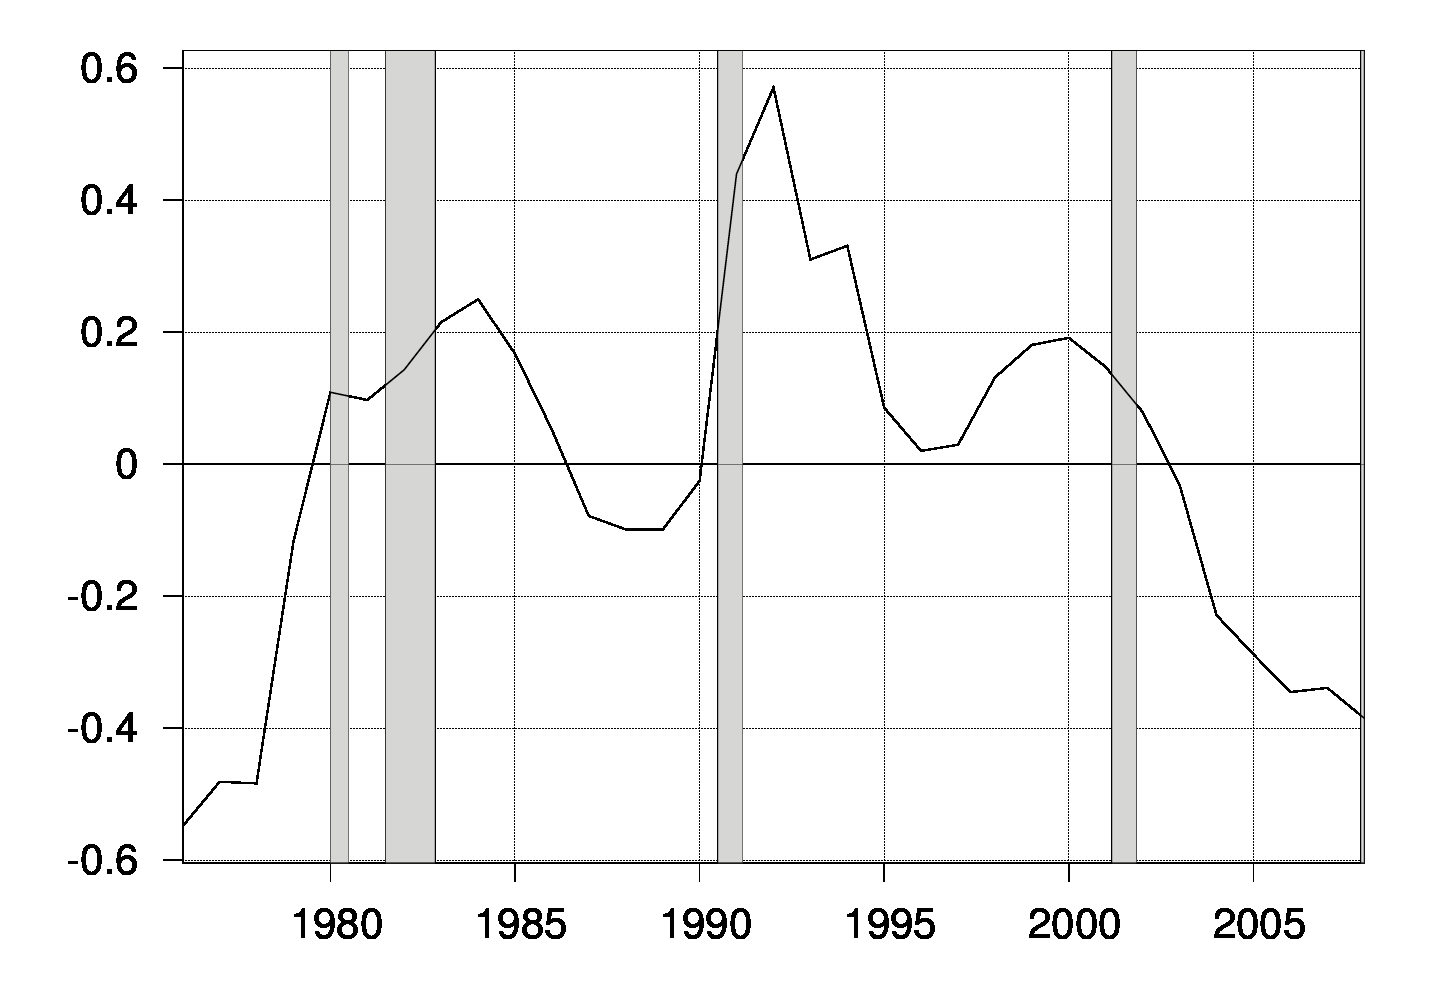
\includegraphics[scale=0.16]{pitchers/salsres.png} & 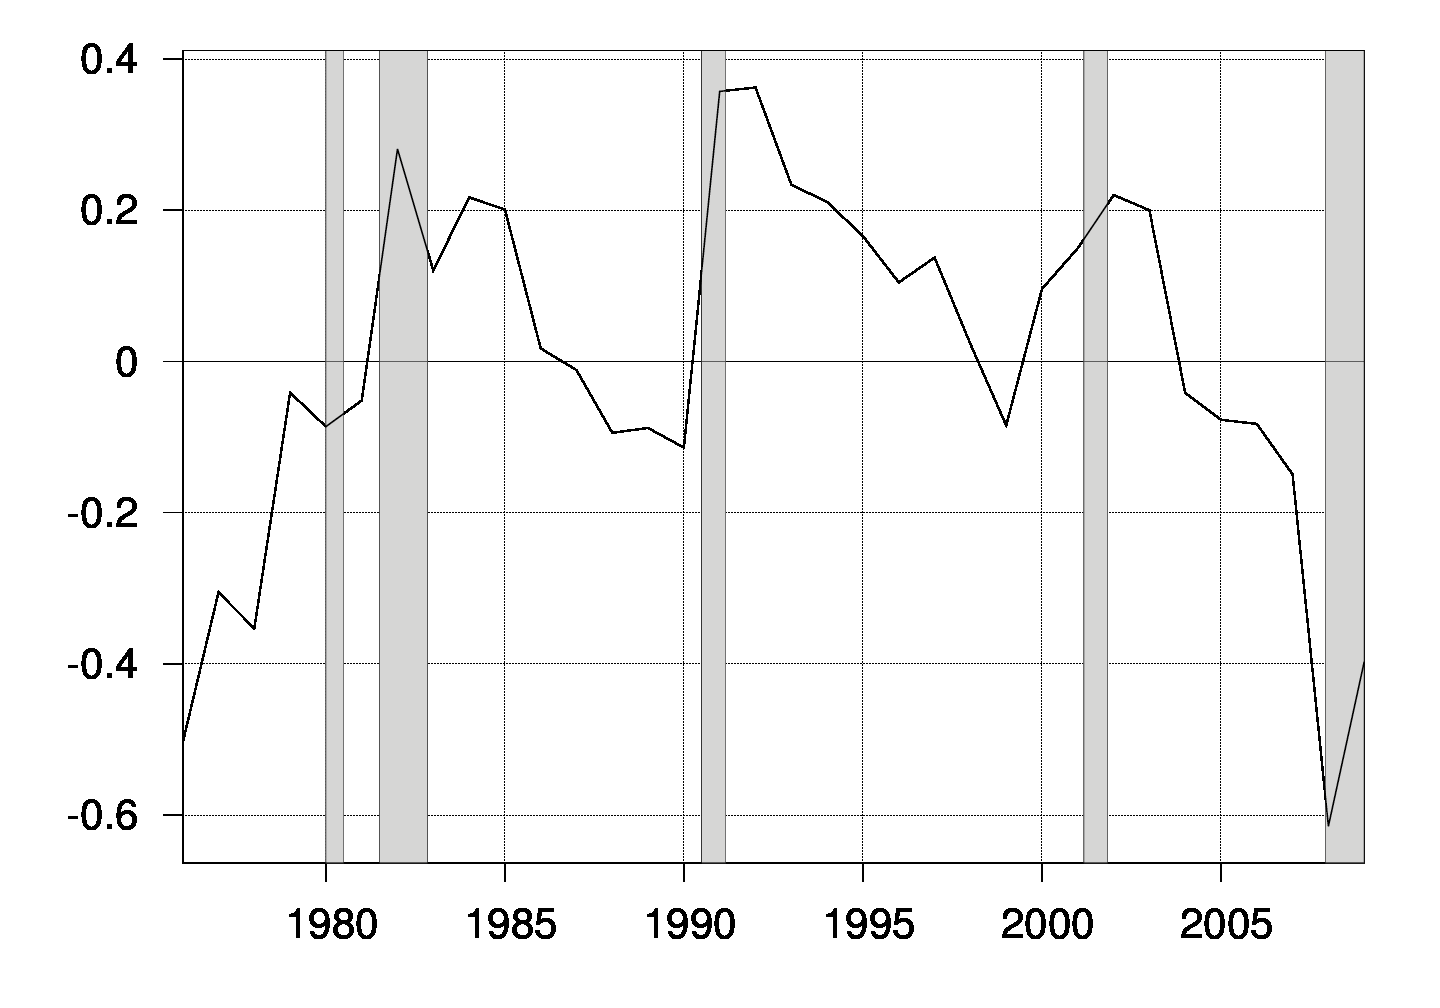
\includegraphics[scale=0.16]{hitters/salsres.png} \\
\multicolumn{2}{c}{Deviation of Log-Salary from Trend} \\
\end{tabular}
\end{center}
\end{figure}

\begin{table} \caption{Pitchers: Ordinary Least Squares (OLS) and Regime Switching Results.}
\begin{center}
\begin{tabular}{l|c|cc|c} 
 Variable & OLS & Regime 1 & Regime 2 & Difference \\ \hline 

 \multirow{2}{*}{Constant} & 1.3318* & 1.6662* & -2.4220* & 4.0882** \\ 
 & (0.7986) & (0.9037) & (1.4418) & (1.7017) \\ [0.4pc]
 \multirow{2}{*}{Time} & 0.0873*** & 0.0864*** & 0.1126*** & -0.0262*** \\ 
 & (0.0019) & (0.0026) & (0.0032) & (0.0042) \\ [0.4pc]
 \multirow{2}{*}{Age} & 0.1623*** & 0.1611*** & 0.1625* & -0.0014  \\ 
 & (0.0539) & (0.0605) & (0.0979) & (0.1152) \\ [0.4pc]
 \multirow{2}{*}{Age Squared} & -0.0033*** & -0.0035*** & -0.0027* & -0.0008  \\ 
 & (0.0009) & (0.0010) & (0.0016) & (0.0020) \\ [0.4pc]
 \multirow{2}{*}{Experience} & 0.3822*** & 0.4043*** & 0.3239*** & 0.0804** \\ 
 & (0.0132) & (0.0139) & (0.0309) & (0.0338) \\ [0.4pc]
 \multirow{2}{*}{Experience Squared} & -0.0115*** & -0.0119*** & -0.0096*** & -0.0024  \\ 
 & (0.0008) & (0.0009) & (0.0018) & (0.0020) \\ [0.4pc]
 \multirow{2}{*}{Earned Run Average} & -0.0602*** & -0.0614*** & 0.0133  & -0.0747*** \\ 
 & (0.0037) & (0.0038) & (0.0149) & (0.0154) \\ [0.4pc]
 \multirow{2}{*}{Wins/Games} & 7.0261*** & 6.9312*** & 12.7643*** & -5.8331*** \\ 
 & (0.3283) & (0.3411) & (1.0284) & (1.0834) \\ [0.4pc]
 \multirow{2}{*}{Saves/Games} & 2.1266*** & 1.9168*** & 3.8812*** & -1.9645*** \\ 
 & (0.2872) & (0.3170) & (0.5672) & (0.6498) \\ [0.4pc]
 \multirow{2}{*}{SO/BB} & 0.0245* & 0.0234* & 0.0653** & -0.0418  \\ 
 & (0.0128) & (0.0137) & (0.0296) & (0.0326) \\ [0.4pc]\hline 
\multirow{2}{*}{p} & - & \multicolumn{2}{c|}{0.9365} & - \\ 
 & & \multicolumn{2}{c|}{(0.9521)} & \\ [0.4pc] 
\multirow{2}{*}{q} & - & \multicolumn{2}{c|}{0.9397} & - \\ 
 & & \multicolumn{2}{c|}{(0.9309)} & \\ \hline 
(Pseudo) $R^2$ & 0.7373 & \multicolumn{2}{c|}{0.7614} & - \\ 
Pseudo $R_{RS/OLS}^2$ & - & \multicolumn{2}{c|}{0.0917} & - \\ \hline
\multicolumn{5}{p{5in}}{\footnotesize{* significant at 10\% level, ** significant at 5\% level, *** Significant at 1\% level.\newline Standard errors in parentheses.  Number of observations = 2581,\newline Number of players = 570, Time period = 1976-2007.}}
\end{tabular}
\end{center}
\end{table}

\begin{table} \caption{Hitters: Ordinary Least Squares (OLS) and Regime Switching Results.}
\begin{center}
\begin{tabular}{l|c|cc|c} 
Variable & OLS & Regime 1 & Regime 2 & Difference \\ \hline 

 \multirow{2}{*}{Constant} & -1.3135* & -1.0324  & -4.7595*** & 3.7271** \\ 
 & (0.7431) & (0.8455) & (1.5537) & (1.7681) \\ [0.4pc]
 \multirow{2}{*}{Time} & 0.0915*** & 0.0889*** & 0.1080*** & -0.0191*** \\ 
 & (0.0017) & (0.0027) & (0.0027) & (0.0038) \\ [0.4pc]
 \multirow{2}{*}{Age} & 0.2803*** & 0.2813*** & 0.3918*** & -0.1105  \\ 
 & (0.0509) & (0.0570) & (0.1050) & (0.1194) \\ [0.4pc]
 \multirow{2}{*}{Age Squared} & -0.0054*** & -0.0055*** & -0.0072*** & 0.0017  \\ 
 & (0.0009) & (0.0010) & (0.0018) & (0.0020) \\ [0.4pc]
 \multirow{2}{*}{Experience} & 0.4308*** & 0.4438*** & 0.3890*** & 0.0549  \\ 
 & (0.0139) & (0.0148) & (0.0304) & (0.0338) \\ [0.4pc]
 \multirow{2}{*}{Experience Squared} & -0.0131*** & -0.0136*** & -0.0103*** & -0.0033  \\ 
 & (0.0009) & (0.0010) & (0.0019) & (0.0021) \\ [0.4pc]
 \multirow{2}{*}{Home Runs} & 0.0088*** & 0.0083*** & 0.0149*** & -0.0066  \\ 
 & (0.0020) & (0.0021) & (0.0044) & (0.0049) \\ [0.4pc]
 \multirow{2}{*}{OPS x AB} & 0.0019*** & 0.0020*** & 0.0014*** & 0.0006** \\ 
 & (0.0001) & (0.0001) & (0.0003) & (0.0003) \\ [0.4pc]\hline 
\multirow{2}{*}{p} & - & \multicolumn{2}{c|}{0.9255} & - \\ 
 & & \multicolumn{2}{c|}{(0.9421)} & \\ [0.4pc] 
\multirow{2}{*}{q} & - & \multicolumn{2}{c|}{0.9566} & - \\ 
 & & \multicolumn{2}{c|}{(0.9533)} & \\ \hline 
(Pseudo) $R^2$ & 0.7283 & \multicolumn{2}{c|}{0.7418} & - \\ 
Pseudo $R_{RS/OLS}^2$ & - & \multicolumn{2}{c|}{0.0497} & - \\ \hline
\multicolumn{5}{p{5in}}{\footnotesize{* significant at 10\% level, ** significant at 5\% level, *** Significant at 1\% level.\newline Standard errors in parentheses.  Number of observations = 3755,\newline Number of players = 732, Time period = 1976-2008.}}
\end{tabular}
\end{center}
\end{table}

\begin{figure}\caption{Smoothed probability labor market is characterized by Regime 2}
\begin{center}
\begin{tabular}{c}
\textbf{Pitchers} \\
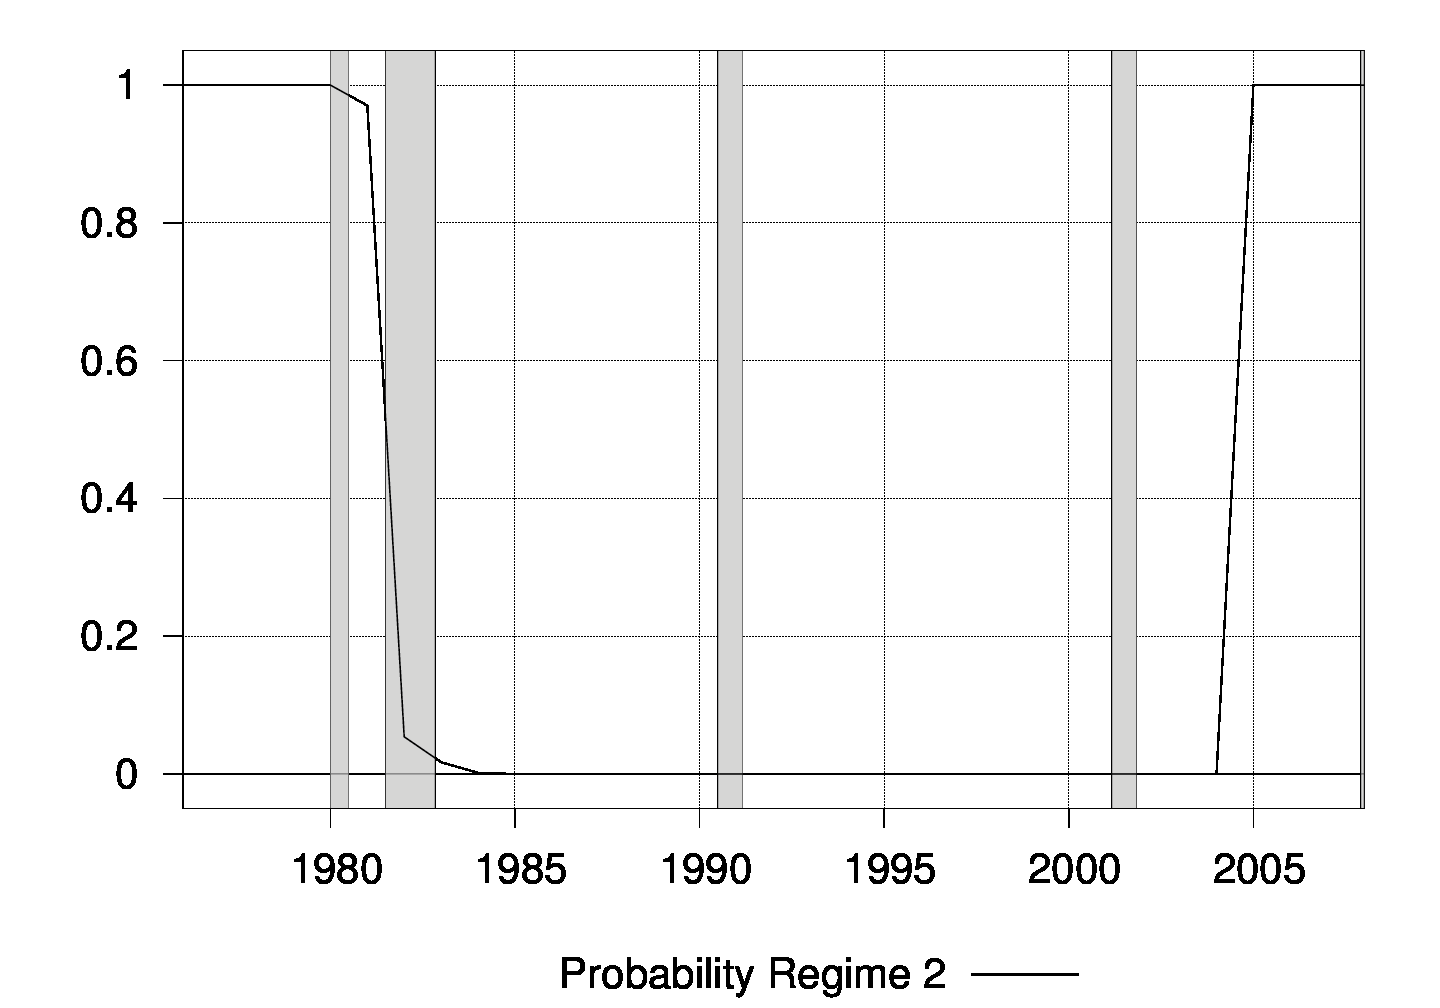
\includegraphics[scale=0.2]{pitchers/regime.png} \\ \\
\textbf{Hitters} \\
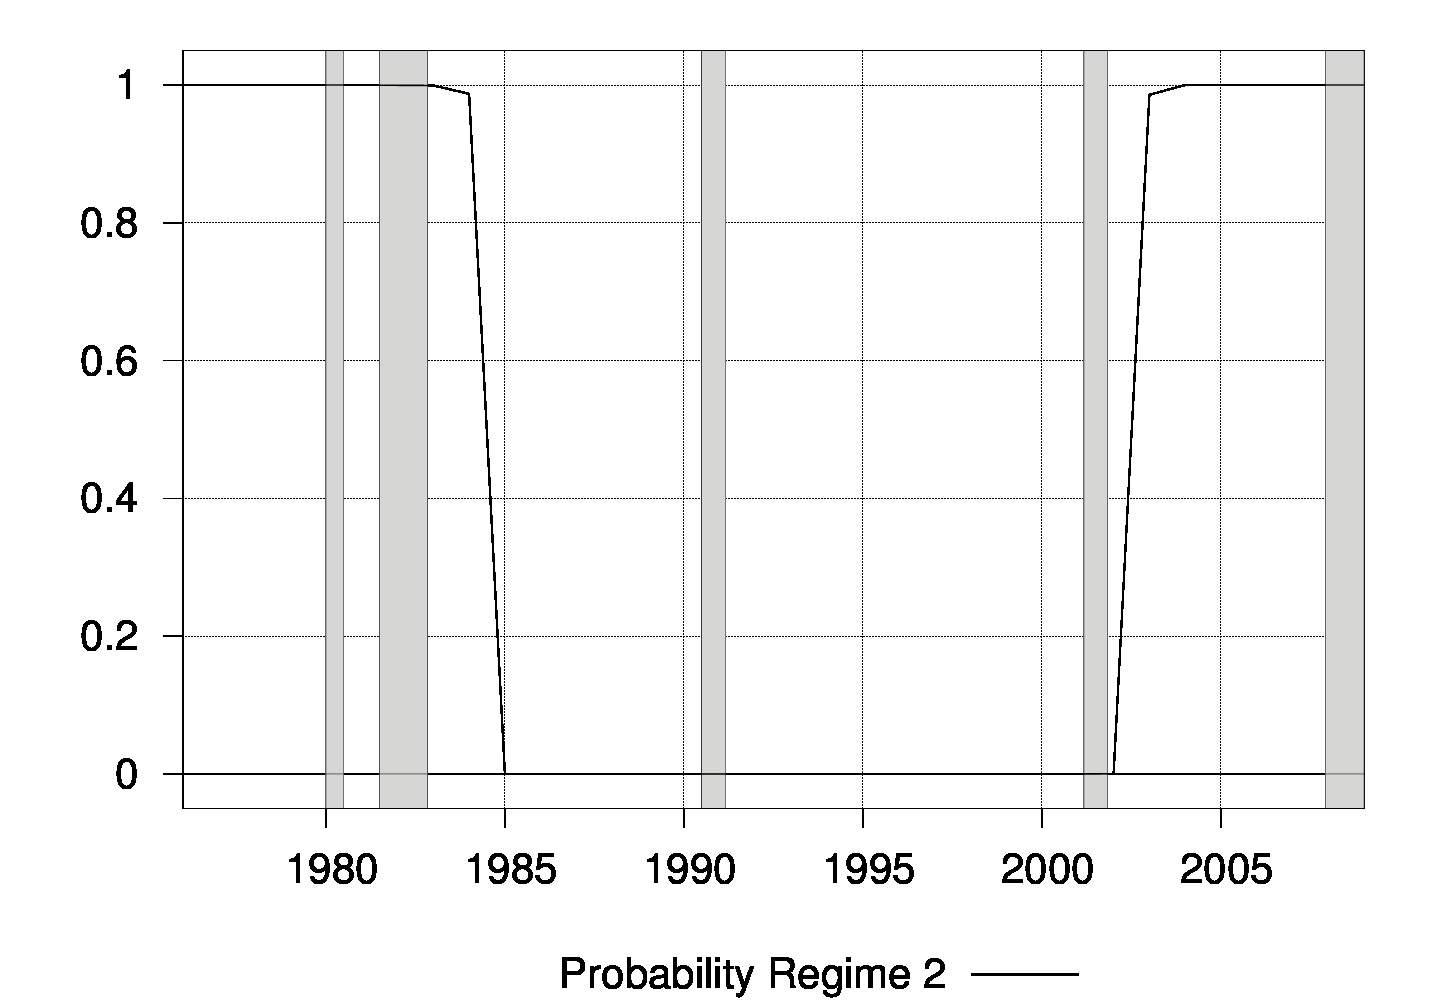
\includegraphics[scale=0.2]{hitters/regime.png} \\
\end{tabular}
\end{center}
\end{figure}

\begin{table}\caption{Labor Market Regime Changes$^1$}\label{tb:regimes}
\begin{center}
\begin{tabular}{ccc}
Regime & Pitchers Time Period & Hitters Time Period \\ \hline
Regime 2 & 1976 - 1981 & 1976 - 1984 \\
Regime 1 & 1982 - 2004 & 1985 - 2002 \\
Regime 2 & 2005 - 2007 & 2003 - 2008 \\
\hline
\multicolumn{2}{p{2.5in}}{$^1$A time period is identified in a given regime if the smoothed probability is greater than 0.5.}
\end{tabular}
\end{center}
\end{table}



\end{document}
